% Manual Código

% Configuración
\documentclass[a4paper,12pt]{book}

\usepackage[utf8]{inputenc}
\usepackage[spanish]{babel}
\usepackage[top=3cm,bottom=3cm,left=3.5cm,right=2cm]{geometry}
\usepackage{fancyhdr}
\usepackage[bookmarksnumbered=true,pdfborder={0 0 0},colorlinks=true,
            linkcolor=blue,urlcolor=blue,citecolor=blue]{hyperref}
\usepackage[final]{pdfpages}
\usepackage[nottoc,notlof]{tocbibind}
\usepackage{multirow}
\usepackage{longtable}
%

% Cabeceras
\pagestyle{fancy}
\headheight 16pt
\lhead{\nouppercase{\rightmark}}
\rhead{\nouppercase{\leftmark}}
%

% Arreglo de los márgenes de las subsecciones
\usepackage[titles]{tocloft}
\cftsetindents{subsection}{1.9em}{3.5em}
\cftsetpnumwidth{1.8em}

% Quitar cabecera y pie de página a las páginas en blanco
\let\origdoublepage\cleardoublepage
\newcommand{\clearemptydoublepage}{%
  \clearpage
{\pagestyle{empty}\origdoublepage}%
}
\let\cleardoublepage\clearemptydoublepage
%

\begin{document}

   \pagenumbering{alph}

   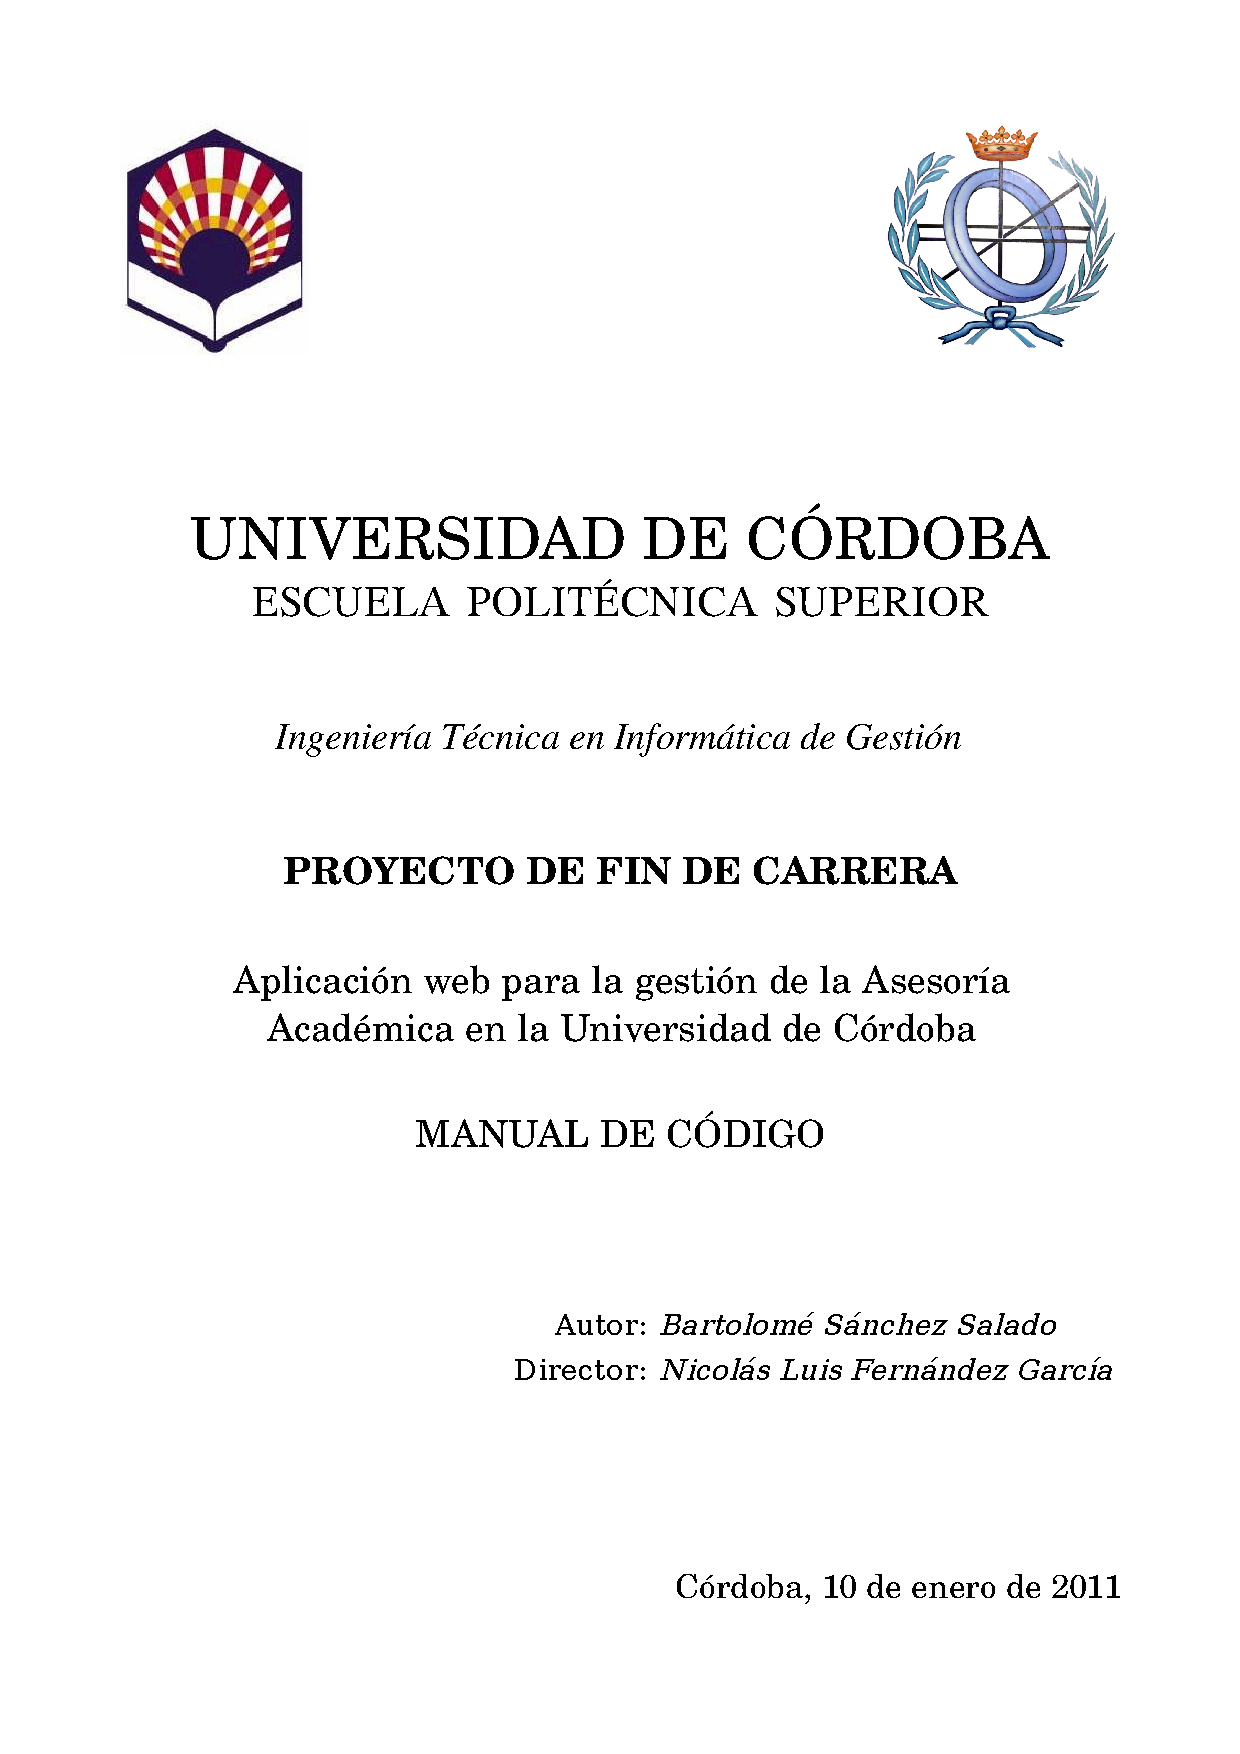
\includepdf[]{Portada/portada_manual_codigo.pdf}
   \cleardoublepage
   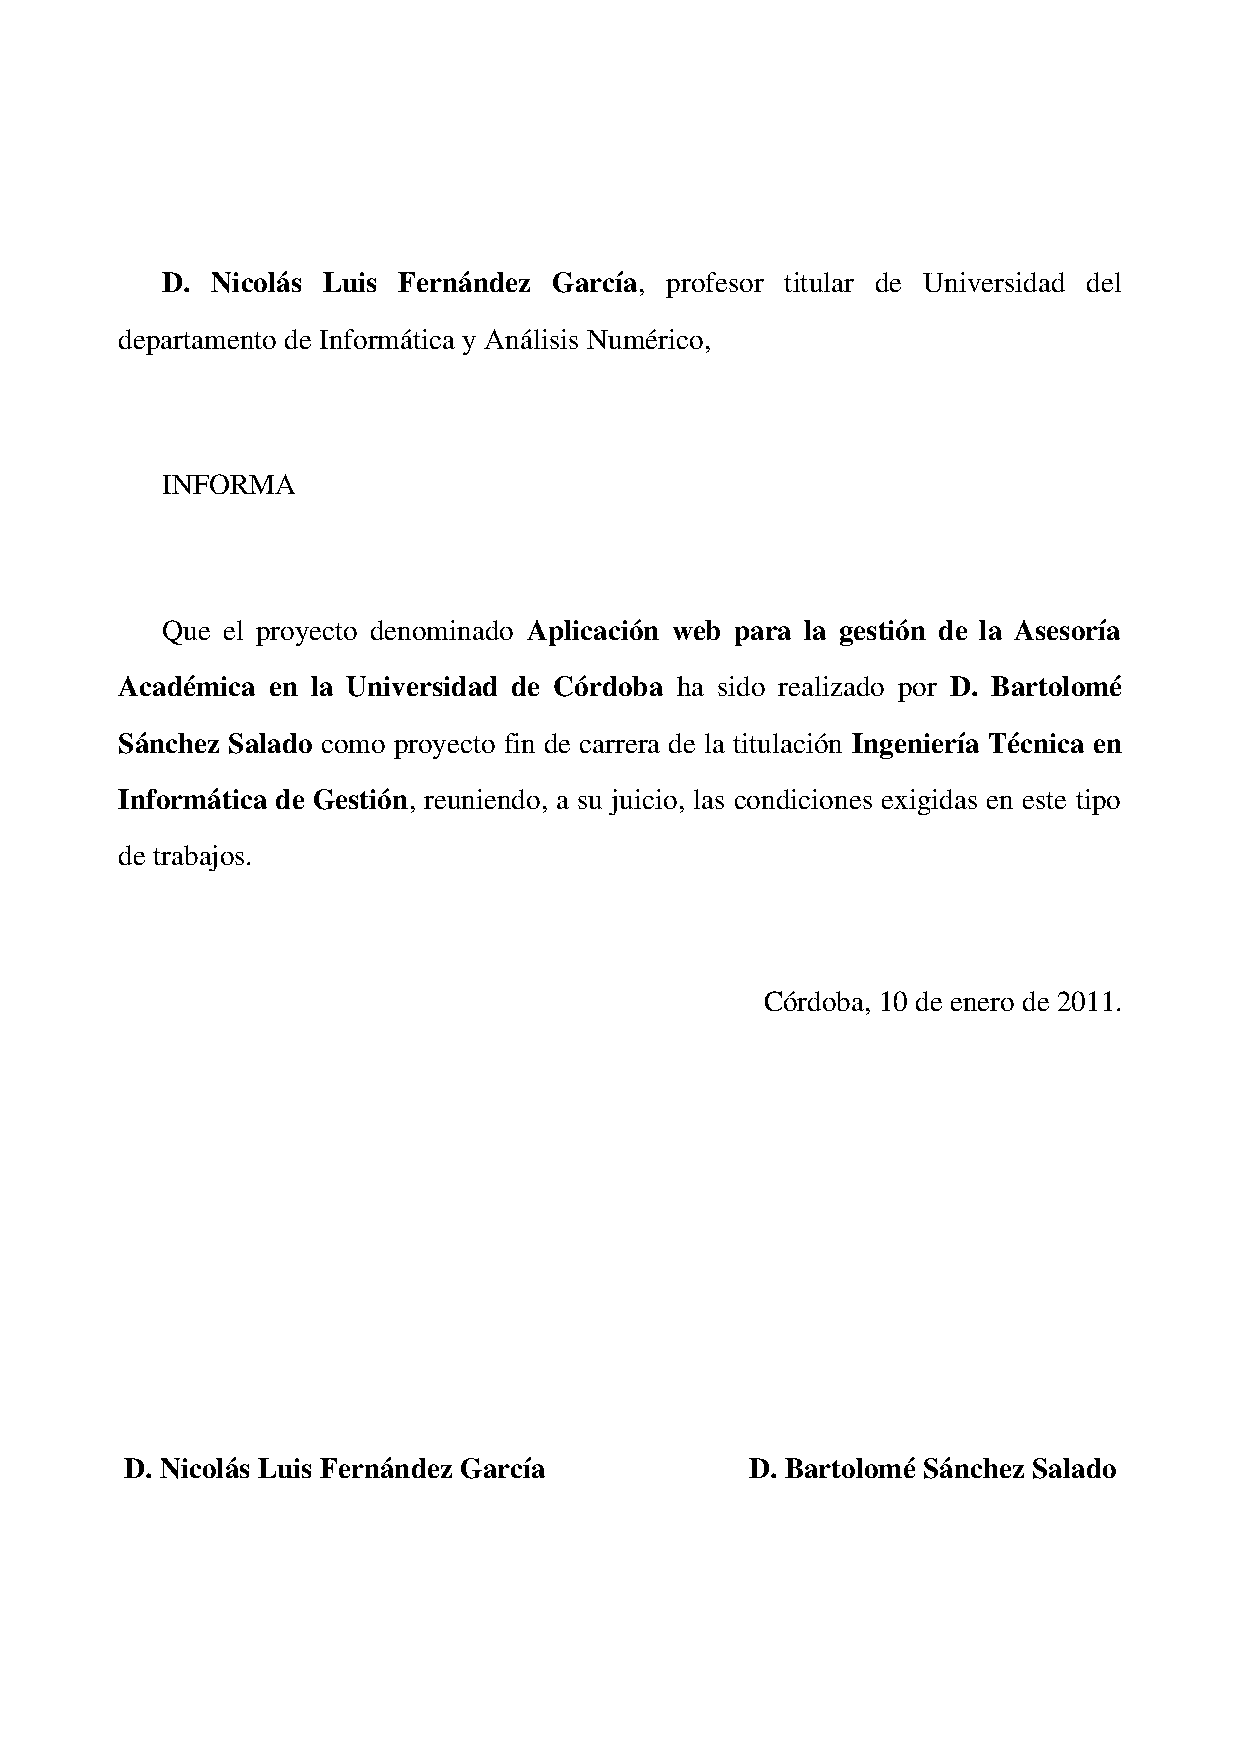
\includepdf[]{Portada/informe_director.pdf}

   \setcounter{page}{0}
   \cleardoublepage

   \pagenumbering{roman}
   \tableofcontents

   \listoffigures

   \chapter{Documentación externa}
    \pagenumbering{arabic}
      \section{Introducción}
      \section{Funcionamiento de la aplicación}
         \subsection{Recursos de software}
         \subsection{Recursos de hardware}
         \subsection{Creación de la aplicación}
      \section{Descripción modular}

   \chapter{Documentación interna}
      \section{Código}

\end{document}